\documentclass[10pt, aspectratio=169]{beamer}

\usepackage{polyglossia}
\usepackage{csquotes}
\usepackage{bm}
\usepackage{datetime}
\usepackage{fontspec}
\usepackage{microtype}
\usepackage{color}
\usepackage{url}
\usepackage{pgfplots}
\usepackage{hyperref}
\usepackage{amsfonts}
\usepackage{amsmath}
\usepackage{amsthm}
\usepackage{subcaption}
\usepackage[backend=biber,style=iso-authoryear,sortlocale=en_US,autolang=other,bibencoding=UTF8]{biblatex}
\usepackage{booktabs}
\usepackage{graphics}
\usepackage{pifont}
\usepackage{ulem}
\usepackage{tikz}

\usepgfplotslibrary{fillbetween}
\usetikzlibrary{patterns}

\addbibresource{zotero.bib}

\setdefaultlanguage{english}
\setmainfont{TeX Gyre Termes}
\usetheme{Boadilla}
\usecolortheme{crane}
\setbeamertemplate{title page}[default][rounded=true,shadow=false]
\setbeamertemplate{section in toc}[ball unnumbered]
\setbeamertemplate{bibliography item}{}

\hypersetup{
	pdfencoding=auto,
	unicode=true,
	citecolor=green,
	filecolor=blue,
	linkcolor=red,
	urlcolor=blue
}

\makeatletter
\newcommand*{\currentSection}{\@currentlabelname}
\makeatother

\newcommand{\mathmat}{\ensuremath{\mathbf}}

\title[Adaptive graph coarsening]
{
	Graph Neural Networks for Adaptive Coarsening of Graphs
}

\newdate{presentation}{24}{11}{2022}
\date[November 2022]{Machine learning seminar 2022, \displaydate{presentation}}

\author[Marek Dědič]
{
	Marek~Dědič\inst{1}\inst{2},
}

\institute[CTU \& Cisco]
{
	\inst{1} Czech Technical University in Prague \and
	\inst{2} Cisco Systems, Inc.
}

% Title card
%\AtBeginSection[]{
	%\begin{frame}
		%\vfill
		%\centering
		%\begin{beamercolorbox}[sep = 8pt,center,shadow = true,rounded = true]{title}
			%\usebeamerfont{title}\insertsectionhead\par%
		%\end{beamercolorbox}
		%\vfill
	%\end{frame}
%}

\AtBeginSection[]{
	\begin{frame}{\currentSection}
		\tableofcontents[currentsection]
	\end{frame}
}

\begin{document}

\begin{frame}
	\titlepage
	\hfill\usebeamerfont{date}\url{marek@dedic.eu}\hspace{1cm}
	\vspace{0.5cm}
\end{frame}

\section{Problem introduction}

\begin{frame}
	\frametitle{Motivation}
	\begin{itemize}
	    \item<1-> Network communication $\to$ cybersecurity
	\end{itemize}
	\scalebox{0.6}{\newcommand\user[2]{
	\begin{scope}[xshift=#1cm, yshift=#2cm]
		\clip (0, 0) circle (0.5);
		\fill[black] (0, 0) circle (0.5);
		\fill[white] (0, 0) circle (0.48);
		\fill[black] (0, -0.675) circle (0.4);
		\fill[black] (0, 0.075) circle (0.24);
  \end{scope}
}

\newcommand\ip[2]{
	\begin{scope}[xshift=#1cm, yshift=#2cm]
		%\rectangle[fill=black, rounded corners=0.2cm] (-0.5, -0.7) -- (0.5, 0.7);
		\draw[fill=black, thick, rounded corners=0.15cm] (-0.3, -0.5) rectangle (0.3, 0.5);
		\draw[fill=white] (0, -0.3) circle (0.1);
		\draw[fill=white, rounded corners=0.07cm] (-0.2, -0.1) rectangle (0.2, 0.0);
		\draw[fill=white, rounded corners=0.07cm] (-0.2, 0.1) rectangle (0.2, 0.2);
		\draw[fill=white, rounded corners=0.07cm] (-0.2, 0.3) rectangle (0.2, 0.4);
  \end{scope}
}

\newcommand\www[2]{
	\begin{scope}[xshift=#1cm, yshift=#2cm]
		\clip (0, 0) circle (0.5);
		\fill[yellow!65!black] (0, 0) circle (0.5);
		\fill[white] (-0.5, -0.175) rectangle (0.5,0.175);
		\node[text=yellow!65!black] at (0,0) {www};
  \end{scope}
}

\newcommand\malwww[2]{
	\begin{scope}[xshift=#1cm, yshift=#2cm]
		\clip (0, 0) circle (0.5);
		\fill[red!65!black] (0, 0) circle (0.5);
		\fill[white] (-0.5, -0.175) rectangle (0.5,0.175);
		\node[text=yellow!65!black] at (0,0) {www};
  \end{scope}
}

\newcommand\wwwline[3]{
	\node[circle, minimum size=1.1cm] (#3) at (0, #1) {};
	\www{0}{#1}
	\node[text width=50mm, align=right] at (-3.5, #1) {#2};
}

\newcommand\malwwwline[3]{
	\node[circle, minimum size=1.1cm] (#3) at (0, #1) {};
	\malwww{0}{#1}
	\node[text width=50mm, align=right] at (-3.5, #1) {#2};
}

\newcommand\userline[2]{
	\node[circle, minimum size=1.1cm] (#2) at (5, #1) {};
	\user{5}{#1}
	\node[text width=50mm, align=left] at (8.5, #1) {#2};
}

\newcommand\ipline[3]{
	\node[circle, minimum size=1.1cm] (#3) at (5, #1) {};
	\ip{5}{#1}
	\node[text width=50mm, align=left] at (8.5, #1) {#2};
}

\begin{tikzpicture}
\uncover<2->{
\node at (-10, 1.2) (x)
{
\begin{tabular}{|c|c|c|c|}
\hline
$\bm{time}$ & $\bm{user}$ & $\bm{domain}$ & $\bm{ip}$ \\
\hline
$t_1$&alice& candidate.com& 1.12.2.3\\
$t_2$&bob& somedomain.ch& 2.7.12.1\\
$t_3$&bob& ransomware.com& 2.7.12.1\\
$t_4$&david& unknown.com & 1.12.2.3\\
$t_5$&bob& evil.com & 1.12.2.3 \\
$t_6$&charlie& candidate.com & 1.12.2.3 \\
$t_7$&bob & somedomain.ch& 2.7.12.1 \\
$t_8$&david& unknown.com & 1.12.2.3\\
\vdots &\vdots &\vdots &\vdots \\
\hline
\end{tabular}
};
}
%{
%$\left\{\begin{array}{c}
%alice, candidate.com, 1.12.2.3\\
%bob, somedomain.ch, 2.7.12.1\\
%bob, ransomware.com, 2.7.12.1\\
%david, unknown.com , 1.12.2.3\\
%bob, evil.com , 1.12.2.3 \\
%charlie, candidate.com , 1.12.2.3 \\
%bob, somedomain.ch, 2.7.12.1 \\
%\dots
%\end{array}\right\}$};
%}
\uncover<3->{
	\malwwwline{-2}{evil.com}{D1};
	\malwwwline{-0.5}{ransomware.com}{D2};
	\wwwline{4}{\textcolor{blue}{candidate.com}}{D5};
	\ipline{-1}{1.12.2.3}{i1}
	\userline{4.2}{Alice};
	\draw (Alice) -- (D1);
  \draw (Alice) -- (D2);
  \draw (i1) -- (D1);
  \draw (Alice) -- (D5);
	\draw (i1) -- (D5);
	\wwwline{1}{unknown.com}{D3};
	\wwwline{2.5}{somedomain.ch}{D4};
	\ipline{-2.2}{2.7.12.1}{i2}
	\userline{0.6}{David};
	\userline{1.8}{Charlie};
	\userline{3}{Bob};
  \draw (Alice) -- (D3);
  \draw (Bob) -- (D1);
  \draw (Bob) -- (D2);
  \draw (Bob) -- (D1);
  \draw (David) -- (D1);
  \draw (i2) -- (D2);
  \draw (Bob) -- (D4);
  \draw (David) -- (D3);
  \draw (Charlie) -- (D4);
  \draw (Charlie) -- (D5);
  \draw (i1) -- (D3);
  \draw (i2) -- (D4);

}
\end{tikzpicture}
}

	\begin{itemize}
	    \item <4-> Goal: identification of malicious domains
	    \item <5-> Currently simple, scalable models
	    \item <5-> State of the art: GNNs
	    \item <6-> Problem -- \alert{complexity} required by GNNs on large graphs
	    \end{itemize}
\end{frame}

\begin{frame}{Problem introduction}
	\begin{itemize}
		\item GNNS on big graphs -- computationally costly and sometimes even unfeasible.
	    \item Suggested solution: compressing the input graph
		\item How much can a graph be coarsened?
		\item Sometimes compressed data \( \implies \) better performace
	\end{itemize}
\end{frame}

\begin{frame}{Main idea}
	\centering
    \begin{tikzpicture}
\tikzset{classA/.style={circle, draw=black, fill=blue!20!yellow}, node distance=1.5cm}
\tikzset{classB/.style={circle, draw=black, fill=blue!20}, node distance=1.5cm}
\tikzset{class0/.style={circle, draw=black, fill=white}, node distance=1.5cm}
  \begin{scope}
    \node[class0] (A) {$\nu_{A}$};
    \node[class0, below right of=A] (B) {$\nu_{B}$};
    \node[class0, below right of=B] (C) {$\nu_{C}$};
    \node[class0, above right of=B] (D) {$\nu_{D}$};
    \node[class0, below right of=D] (E) {$\nu_{E}$};
    \draw [-] (A) -- (B) ;
    \draw [-] (A) -- (D) ;
    \draw [-] (C) -- (D) ;
    \draw [-] (D) -- (E) ; 
    \draw [-] (C) -- (E) ;  
    \draw [-] (C) -- (B) ;    
    \draw [-] (D) -- (B) ;
    \draw[->, thick] ([xshift=6ex] E.center) -- ([xshift=15ex] E.center) node [pos=0.5, above] (oGNN) {GNN}; \
    \node[below of=oGNN, node distance=3ex]{\alert{infeasible}};
    \uncover<2->{
        \draw[->, thick] ([yshift=-4ex] C.center) -- ([yshift=-10ex] C.center) node [pos=0.5, right] (ocoars) {Coarsening};
    }
  \end{scope}

  \begin{scope}[xshift=7.2cm, yshift=0cm]
    \node[classA] (A) {$\nu_{A}$};
    \node[classB, below right of=A] (B) {$\nu_{B}$};
    \node[classB, below right of=B] (C) {$\nu_{C}$};
    \node[classB, above right of=B] (D) {$\nu_{D}$};
    \node[classB, below right of=D] (E) {$\nu_{E}$};
    \draw [-] (A) -- (B) ;
    \draw [-] (A) -- (D) ;
    \draw [-] (C) -- (D) ;
    \draw [-] (D) -- (E) ; 
    \draw [-] (C) -- (E) ;  
    \draw [-] (C) -- (B) ;    
    \draw [-] (D) -- (B) ;   
    % \uncover<3->{\node[above of=D, node distance=4ex]{{\color{green} good performance}};}    
  \end{scope} 

\uncover<2->{
    \begin{scope}[yshift=-4.75cm, xshift=0.1cm]
        \node[class0] (AB) {$\nu_{AB}$};
    \node[class0, right of=AB] (CD) {$\nu_{CD}$};
    \node[class0, right of=CD] (E) {$\nu_{E}$};
    \draw [-] (AB) -- (CD);
    \draw [-] (CD) -- (E); 
    \uncover<3->{
        \draw[->, thick] ([xshift=6ex] E.center) -- ([xshift=15ex] E.center) node [pos=0.5, above] (oGNN) {GNN};
    }
    % \uncover<2->{\node[below of=oGNN, node distance=3ex]{{\color{green} simplified}};}
  \end{scope}
  }
  
  \uncover<3->{
    \begin{scope}[yshift=-4.75cm, xshift=8cm]
        \node[classA] (AB) {$\nu_{AB}$};
    \node[classB, right of=AB] (CD) {$\nu_{CD}$};
    \node[classB, right of=CD] (E) {$\nu_{E}$};
    \draw [-] (AB) -- (CD);
    \draw [-] (CD) -- (E);
    % \uncover<3->{\node[below of=CD, node distance=4ex]{{\color{red} worse performance}};}
    \end{scope}
}
 \end{tikzpicture}

\end{frame}

\section{Prior art - the HARP method}

\begin{frame}{HARP - learning on coarser graphs}
	\begin{itemize}
		\item HARP - a method for pretraining on simplified graphs
		\item Simplified graphs as depicted bellow
		\item Embedding trained first on the coarser graph
	\end{itemize}
	\begin{figure}
		\centering
		\begin{subfigure}[t]{0.38\textwidth}
			\centering
			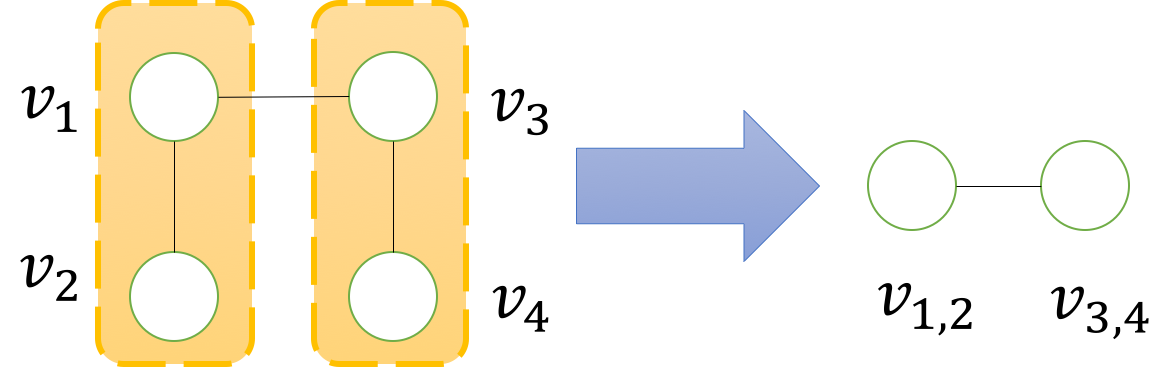
\includegraphics[width=\textwidth]{images/edge_collapsing.png}
			\caption{Edge collapsing}
		\end{subfigure}
		\hspace{2em}
		\begin{subfigure}[t]{0.38\textwidth}
			\centering
			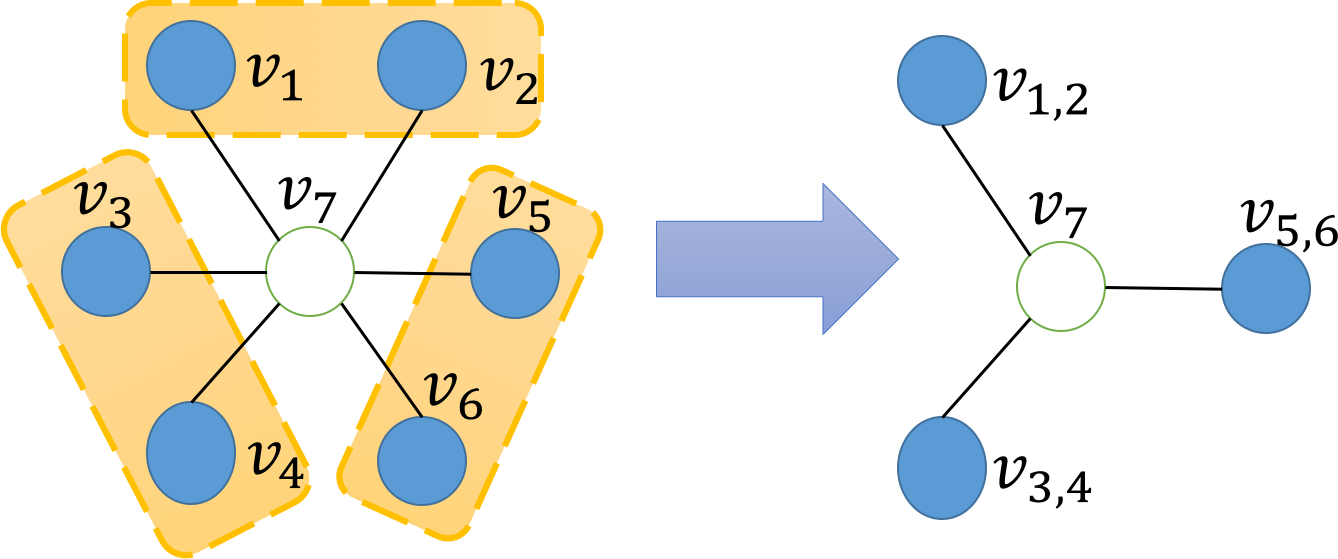
\includegraphics[width=\textwidth]{images/star_collapsing.png}
			\caption{Star collapsing}
		\end{subfigure}
		\caption{HARP coarsening algorithm. \footnote{Images from \cite{chen_harp_2018}.}}
	\end{figure}
\end{frame}

\begin{frame}{HARP pipeline overview}
	\begin{figure}
		\centering
		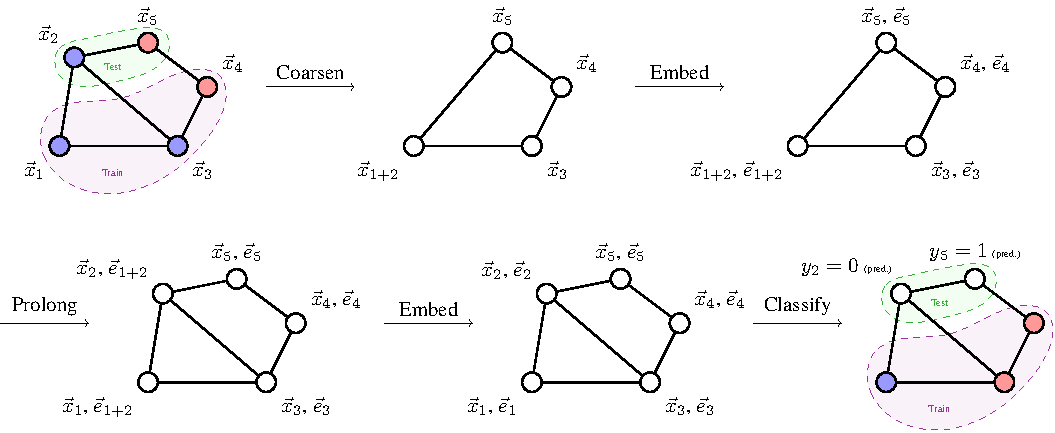
\includegraphics[width=\textwidth]{images/harp-overview/harp-overview.pdf}
	\end{figure}
\end{frame}

\begin{frame}{Deep HARP}
	\begin{figure}
		\centering
		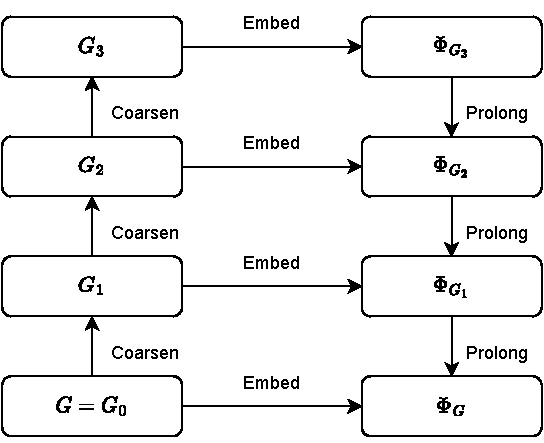
\includegraphics[width=0.5\textwidth]{images/deep-harp/deep-harp.pdf}
	\end{figure}
\end{frame}

\section{The performance-complexity trade-off problem}

\begin{frame}{Main idea}
	\centering
    \begin{tikzpicture}
\tikzset{classA/.style={circle, draw=black, fill=blue!20!yellow}, node distance=1.5cm}
\tikzset{classB/.style={circle, draw=black, fill=blue!20}, node distance=1.5cm}
\tikzset{class0/.style={circle, draw=black, fill=white}, node distance=1.5cm}
  \begin{scope}
    \node[class0] (A) {$\nu_{A}$};
    \node[class0, below right of=A] (B) {$\nu_{B}$};
    \node[class0, below right of=B] (C) {$\nu_{C}$};
    \node[class0, above right of=B] (D) {$\nu_{D}$};
    \node[class0, below right of=D] (E) {$\nu_{E}$};
    \draw [-] (A) -- (B) ;
    \draw [-] (A) -- (D) ;
    \draw [-] (C) -- (D) ;
    \draw [-] (D) -- (E) ; 
    \draw [-] (C) -- (E) ;  
    \draw [-] (C) -- (B) ;    
    \draw [-] (D) -- (B) ;
    \draw[->, thick] ([xshift=6ex] E.center) -- ([xshift=15ex] E.center) node [pos=0.5, above] (oGNN) {GNN}; \
    \node[below of=oGNN, node distance=3ex]{\alert{infeasible}};
    \uncover<2->{
        \draw[->, thick] ([yshift=-4ex] C.center) -- ([yshift=-10ex] C.center) node [pos=0.5, right] (ocoars) {Coarsening};
    }
  \end{scope}

  \begin{scope}[xshift=7.2cm, yshift=0cm]
    \node[classA] (A) {$\nu_{A}$};
    \node[classB, below right of=A] (B) {$\nu_{B}$};
    \node[classB, below right of=B] (C) {$\nu_{C}$};
    \node[classB, above right of=B] (D) {$\nu_{D}$};
    \node[classB, below right of=D] (E) {$\nu_{E}$};
    \draw [-] (A) -- (B) ;
    \draw [-] (A) -- (D) ;
    \draw [-] (C) -- (D) ;
    \draw [-] (D) -- (E) ; 
    \draw [-] (C) -- (E) ;  
    \draw [-] (C) -- (B) ;    
    \draw [-] (D) -- (B) ;   
    % \uncover<3->{\node[above of=D, node distance=4ex]{{\color{green} good performance}};}    
  \end{scope} 

\uncover<2->{
    \begin{scope}[yshift=-4.75cm, xshift=0.1cm]
        \node[class0] (AB) {$\nu_{AB}$};
    \node[class0, right of=AB] (CD) {$\nu_{CD}$};
    \node[class0, right of=CD] (E) {$\nu_{E}$};
    \draw [-] (AB) -- (CD);
    \draw [-] (CD) -- (E); 
    \uncover<3->{
        \draw[->, thick] ([xshift=6ex] E.center) -- ([xshift=15ex] E.center) node [pos=0.5, above] (oGNN) {GNN};
    }
    % \uncover<2->{\node[below of=oGNN, node distance=3ex]{{\color{green} simplified}};}
  \end{scope}
  }
  
  \uncover<3->{
    \begin{scope}[yshift=-4.75cm, xshift=8cm]
        \node[classA] (AB) {$\nu_{AB}$};
    \node[classB, right of=AB] (CD) {$\nu_{CD}$};
    \node[classB, right of=CD] (E) {$\nu_{E}$};
    \draw [-] (AB) -- (CD);
    \draw [-] (CD) -- (E);
    % \uncover<3->{\node[below of=CD, node distance=4ex]{{\color{red} worse performance}};}
    \end{scope}
}
 \end{tikzpicture}

\end{frame}

\begin{frame}{Deep HARP}
	\begin{figure}
		\centering
		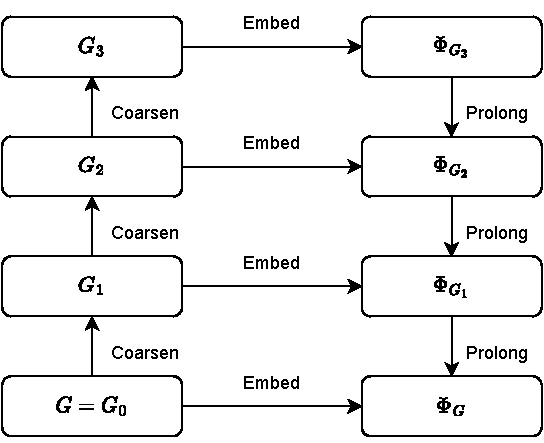
\includegraphics[width=0.5\textwidth]{images/deep-harp/deep-harp.pdf}
	\end{figure}
\end{frame}

\begin{frame}{Complexity performance trade-off}
	\begin{tikzpicture}[xscale=1.2]
\tikzset{point/.style={circle, fill=black, draw=black, inner sep=1pt, minimum size=1ex}}
\tikzset{b/.style={rectangle, fill=black, draw=black, inner sep=1pt, minimum size=1ex}}
\draw[->] (0,0) -- (7,0) node [pos=1, yshift=-2ex,, fill=white, inner sep=2px] {$C$};
\draw[->] (0,0) -- (0,5) node [pos=1, xshift=-2ex, fill=white, inner sep=2px] {$P$};

\node[point] at (1,1) (p1) {};
\node[above of=p1, node distance=3ex] {$G_5$};
\node[point] at (3,2) (p2) {}; \node[above of=p2, node distance=3ex] {$G_4$};
\node[point] at (4,3) (p3) {};
\node[above of=p3, node distance=3ex] {$G_3$};
\node[point] at (5,3.5) (p4) {};
\node[above of=p4, node distance=3ex] {$G_2$};
\node[point] at (6,4) (p5) {};
\node[above of=p5, node distance=3ex] {$G_1$};
\uncover<2>{
\draw[ultra thick] (4.5, 0.1) -- (4.5, -0.1) node [pos=1, yshift=-1.5ex] (CM) {$C_m$};
\draw[->, ultra thick, shorten >=0.5ex, color=blue] (4.5, 0) -- (4.5, 3.25);
\draw[->, ultra thick,shorten >=0.5ex, color=blue] (4.5, 3.25) -- (4, 3);
\draw[->, ultra thick,shorten >=0.5ex, color=blue] (4, 3) -- (0.1, 3);
\draw[ultra thick] (0.1, 3) -- (-0.1, 3) node [pos=1, xshift=-1.5ex] {$P_3$};
\node[below of=CM, node distance=4ex, color=blue] {Achieving best performance $P_3$ for complexity $C_m$.};
}
\uncover<3>{
\draw[ultra thick] (0.1, 1.5) -- (-0.1, 1.5) node [pos=1, xshift=-1.5ex] {$P_m$};
\draw[->, shorten >=0.5ex,
ultra thick,color=green!50!black] (0, 1.5) -- (2, 1.5);
\draw[->, shorten >=0.5ex, ultra thick, color=green!50!black] (2, 1.5) -- (3, 2);
\draw[->, shorten >=0.5ex,
ultra thick,color=green!50!black] (3, 2) -- (3, 0.1);
\draw[ultra thick] (3, 0.1) -- (3,-0.1) node [pos=1, yshift=-1.5ex]  {$C_4$};
\node[below of=CM, node distance=4ex, color=green!50!black] {The least complexity ($C_4$) with performance at least  $P_m$.};
}

\draw[-] (p1) -- (p2) -- (p3) -- (p4) -- (p5);
\end{tikzpicture}

\end{frame}

\begin{frame}{Performance \& Complexity}
	\begin{itemize}
		\item Performance = classification accuracy
	    \item Usually time \& memory complexity
        \item In business, time translates to cost
        \begin{itemize}
            \item More interpretable
            \item Monthly budget \$100, AWS EKS costs \$0.33/hour
            \item Therefore daily run can take 10 hours $\to$ select graph size accordingly
        \end{itemize}
		\item For simplicity, complexity = node count
    \end{itemize}
\end{frame}

\section{Adaptive prolongation}

\begin{frame}{Adaptive prolongation}
	\begin{itemize}
		\item Graph prolongation (de-coarsening) micro-stepping
		\item Guiding the prolongation based on local properties
		\item Possibly results in different \enquote{model resolution} in different parts of the graph
		\item Evaluation -- Training a classifier in each (micro) step
	\end{itemize}
\end{frame}

\begin{frame}{Adaptive prolongation}
	\begin{figure}
		\centering
		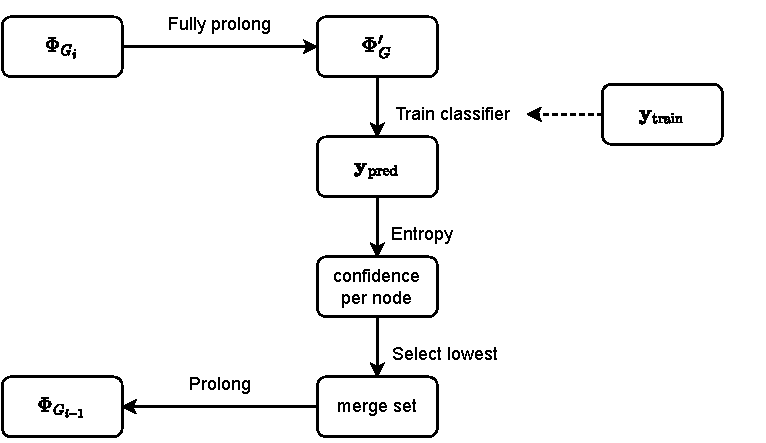
\includegraphics[width=0.8\textwidth]{images/adaptive-prolongation/adaptive-prolongation.pdf}
	\end{figure}
\end{frame}

\begin{frame}{Adaptive prolongation - experimental verification}
	\begin{figure}
		\centering
		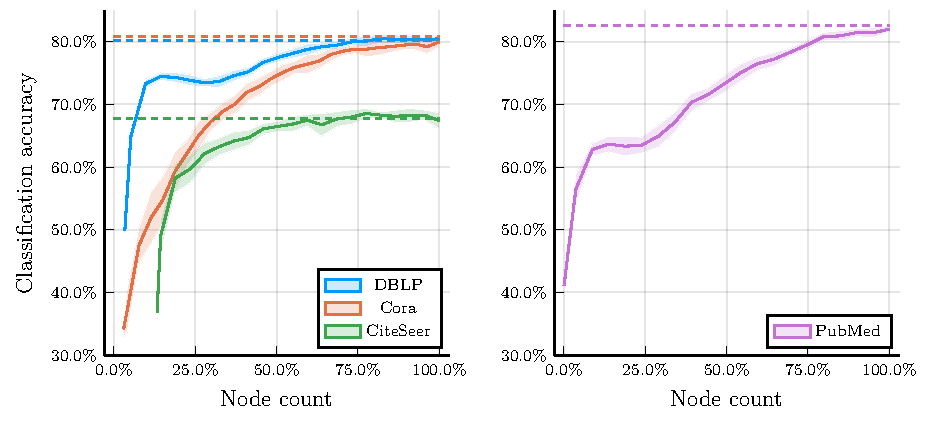
\includegraphics[width=0.9\textwidth]{images/adaptive-coarsening/adaptive-coarsening.pdf}
		\caption{Prediction accuracy with guided prolongation.}
	\end{figure}
\end{frame}

\section{Alternative approaches to coarsening}

\begin{frame}{HARP coarsening}
	\begin{figure}
		\centering
		\begin{subfigure}[t]{0.38\textwidth}
			\centering
			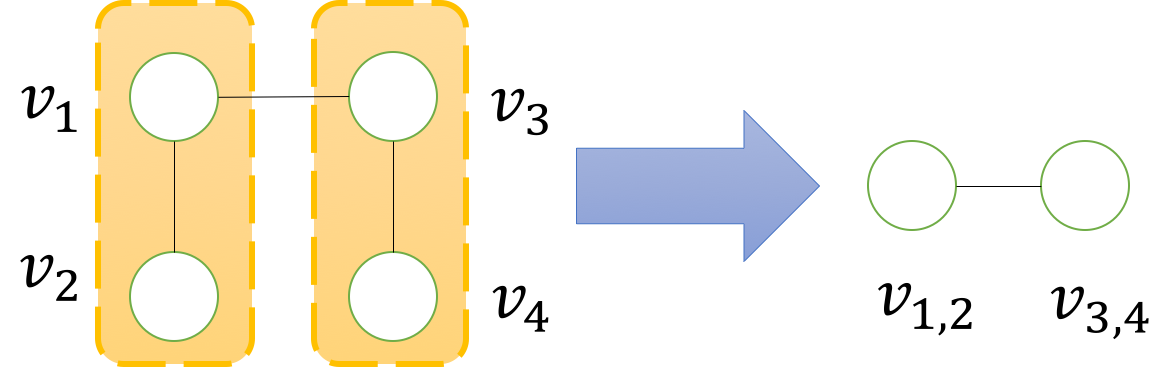
\includegraphics[width=\textwidth]{images/edge_collapsing.png}
			\caption{Edge collapsing}
		\end{subfigure}
		\hspace{2em}
		\begin{subfigure}[t]{0.38\textwidth}
			\centering
			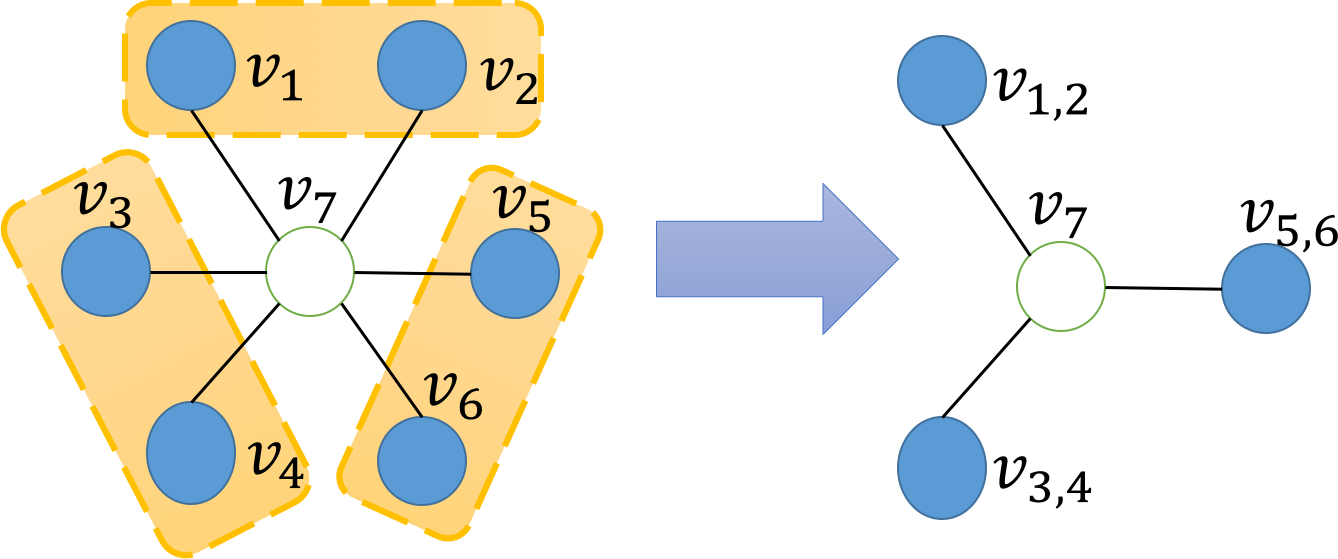
\includegraphics[width=\textwidth]{images/star_collapsing.png}
			\caption{Star collapsing}
		\end{subfigure}
		\caption{HARP coarsening algorithm. \footnote{Images from \cite{chen_harp_2018}.}}
	\end{figure}
\end{frame}

\begin{frame}{Diffusion-based coarsening}
	\begin{itemize}
		\item Creating a new edge matrix \( \hat{\mathmat{S}} \)
		\item Contracting edges \( E \left( G_{\hat{\mathmat{S}}} \right) \cap E \left( G \right) \)
		\item \( \hat{\mathmat{S}} = \sum_{k = 1}^\infty \theta_k \mathmat{T}^k \)
	\end{itemize}
\end{frame}

\begin{frame}{Diffusion-based coarsening}
	\begin{itemize}
		\item \( \hat{\mathmat{S}} = \sum_{k = 1}^\infty \theta_k \mathmat{T}^k \)
		\item Personalized PageRank
		\begin{itemize}
			\item \( \mathmat{T} = \mathmat{A} \mathmat{D}^{-1} \)
			\item \( \theta_k = \alpha \left( 1 - \alpha \right)^k \)
		\end{itemize}
		\item Heat kernel
		\begin{itemize}
			\item \( \mathmat{T} = \mathmat{A} \mathmat{D}^{-1} \)
			\item \( \theta_k = e^{-t} \frac{t^k}{k!} \)
		\end{itemize}
	\end{itemize}
\end{frame}

\begin{frame}{Evolved coarsening}
	\begin{itemize}
		\item A set of atomic coarsenings
		\item A coarsening candidate = sequence of atomic coarsenings
		\item Evolved using a simple genetic algorithm
	\end{itemize}
\end{frame}

\begin{frame}{Experimental comparison of coarsening approaches}
	\begin{figure}
		\centering
		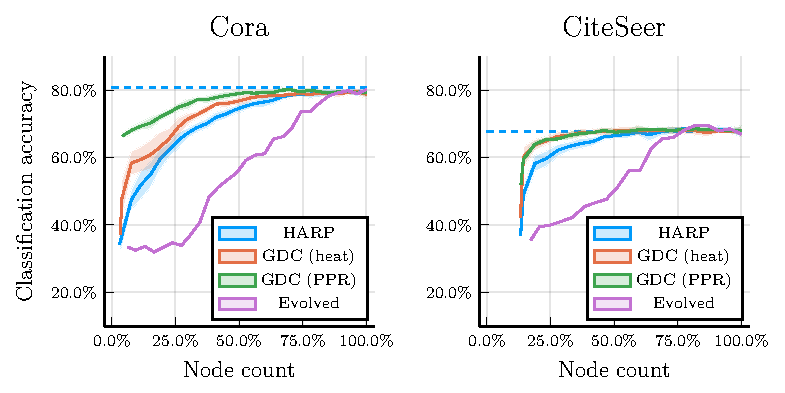
\includegraphics[width=\textwidth]{images/coarsening-algorithms/coarsening-algorithms.pdf}
		\caption{Prediction accuracy with different algorithms.}
	\end{figure}
\end{frame}

\section{Conclusion}

\begin{frame}{Conclusion}
	\centering
	\begin{itemize}
		\item Studying GNN behaviour while coarsening a graph
		\item The adaptive prolongation approach -- a way of studying such behaviour in detail.
		\item 3 alternative coarsening strategies
		\item A new re-formalization of HARP, allowing for a more general approach to graph coarsening
		\item HARP as a framework for graph reduction
	\end{itemize}
\end{frame}

\begin{frame}{Future work}
	\centering
	\begin{itemize}
		\item Investigate more datasets
		\item Surrogate metric for adaptive prolongation
		\item More thorough exploration of evolved coarsenings
	\end{itemize}
\end{frame}

\section{Direct adaptive coarsening}

\begin{frame}{Main idea}
	\centering
    \begin{tikzpicture}
\tikzset{classA/.style={circle, draw=black, fill=blue!20!yellow}, node distance=1.5cm}
\tikzset{classB/.style={circle, draw=black, fill=blue!20}, node distance=1.5cm}
\tikzset{class0/.style={circle, draw=black, fill=white}, node distance=1.5cm}
  \begin{scope}
    \node[class0] (A) {$\nu_{A}$};
    \node[class0, below right of=A] (B) {$\nu_{B}$};
    \node[class0, below right of=B] (C) {$\nu_{C}$};
    \node[class0, above right of=B] (D) {$\nu_{D}$};
    \node[class0, below right of=D] (E) {$\nu_{E}$};
    \draw [-] (A) -- (B) ;
    \draw [-] (A) -- (D) ;
    \draw [-] (C) -- (D) ;
    \draw [-] (D) -- (E) ; 
    \draw [-] (C) -- (E) ;  
    \draw [-] (C) -- (B) ;    
    \draw [-] (D) -- (B) ;
    \draw[->, thick] ([xshift=6ex] E.center) -- ([xshift=15ex] E.center) node [pos=0.5, above] (oGNN) {GNN}; \
    \node[below of=oGNN, node distance=3ex]{\alert{infeasible}};
    \uncover<2->{
        \draw[->, thick] ([yshift=-4ex] C.center) -- ([yshift=-10ex] C.center) node [pos=0.5, right] (ocoars) {Coarsening};
    }
  \end{scope}

  \begin{scope}[xshift=7.2cm, yshift=0cm]
    \node[classA] (A) {$\nu_{A}$};
    \node[classB, below right of=A] (B) {$\nu_{B}$};
    \node[classB, below right of=B] (C) {$\nu_{C}$};
    \node[classB, above right of=B] (D) {$\nu_{D}$};
    \node[classB, below right of=D] (E) {$\nu_{E}$};
    \draw [-] (A) -- (B) ;
    \draw [-] (A) -- (D) ;
    \draw [-] (C) -- (D) ;
    \draw [-] (D) -- (E) ; 
    \draw [-] (C) -- (E) ;  
    \draw [-] (C) -- (B) ;    
    \draw [-] (D) -- (B) ;   
    % \uncover<3->{\node[above of=D, node distance=4ex]{{\color{green} good performance}};}    
  \end{scope} 

\uncover<2->{
    \begin{scope}[yshift=-4.75cm, xshift=0.1cm]
        \node[class0] (AB) {$\nu_{AB}$};
    \node[class0, right of=AB] (CD) {$\nu_{CD}$};
    \node[class0, right of=CD] (E) {$\nu_{E}$};
    \draw [-] (AB) -- (CD);
    \draw [-] (CD) -- (E); 
    \uncover<3->{
        \draw[->, thick] ([xshift=6ex] E.center) -- ([xshift=15ex] E.center) node [pos=0.5, above] (oGNN) {GNN};
    }
    % \uncover<2->{\node[below of=oGNN, node distance=3ex]{{\color{green} simplified}};}
  \end{scope}
  }
  
  \uncover<3->{
    \begin{scope}[yshift=-4.75cm, xshift=8cm]
        \node[classA] (AB) {$\nu_{AB}$};
    \node[classB, right of=AB] (CD) {$\nu_{CD}$};
    \node[classB, right of=CD] (E) {$\nu_{E}$};
    \draw [-] (AB) -- (CD);
    \draw [-] (CD) -- (E);
    % \uncover<3->{\node[below of=CD, node distance=4ex]{{\color{red} worse performance}};}
    \end{scope}
}
 \end{tikzpicture}

\end{frame}

\begin{frame}{HARP pipeline overview}
	\begin{figure}
		\centering
		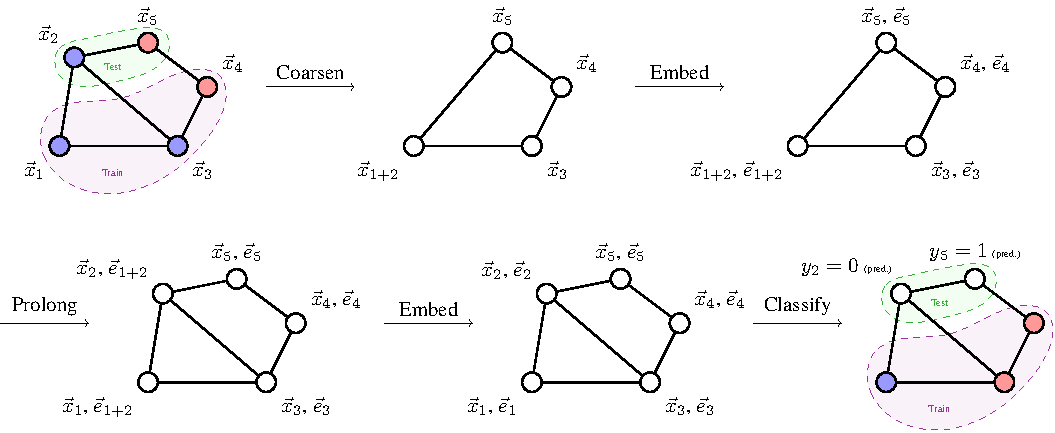
\includegraphics[width=\textwidth]{images/harp-overview/harp-overview.pdf}
	\end{figure}
\end{frame}

\begin{frame}{Direct pipeline}
	\begin{figure}
		\centering
		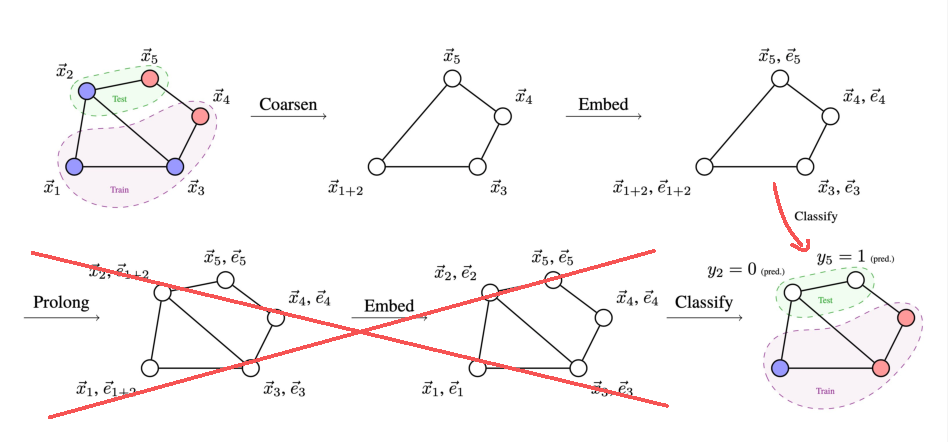
\includegraphics[width=\textwidth]{images/harp-overview-edit.pdf}
	\end{figure}
\end{frame}

\begin{frame}{Details}
    \begin{itemize}
        \item Base model $\to$ posterior for all nodes
        \item Similarity measure
        \item Edge contraction $\to$ graph sequence
        \item GNN on each graph with label propagation
    \end{itemize}
    \vspace{1cm}
	\centering
    \scalebox{0.75}{\begin{tikzpicture}
\tikzset{classA/.style={circle, draw=black, fill=blue!20!yellow}, node distance=1.5cm}
\tikzset{classB/.style={circle, draw=black, fill=blue!20}, node distance=1.5cm}
\tikzset{classX/.style={circle, draw=black, fill=red!20}, node distance=1.5cm}
  \begin{scope}
    \node[classA] (A) {$\nu_{A}$};
    \node[classA, below right of=A] (B) {$\nu_{B}$};
    \node[classB, below right of=B] (C) {$\nu_{C}$};
    \node[classB, above right of=B] (D) {$\nu_{D}$};
    \node[classB, below right of=D] (E) {$\nu_{E}$};
    \draw [-] (A) -- (B) node [midway, fill=white, inner sep=0px] {1};
    \draw [-] (A) -- (D) node [midway, fill=white, inner sep=0px] {5};
    \draw [-] (C) -- (D) node [midway, fill=white, inner sep=0px] {2};
    \draw [-] (D) -- (E) node [midway, fill=white, inner sep=0px] {3}; 
    \draw [-] (C) -- (E) node [midway, fill=white, inner sep=0px] {4};  
    \draw [-] (C) -- (B) node [midway, fill=white, inner sep=0px] {6};    
    \draw [-] (D) -- (B) node [midway, fill=white, inner sep=0px] {7};
    \draw[->, thick] ([xshift=3ex] E.center) -- ([xshift=5ex] E.center);
    \node [below of=C, node distance=4ex] {$G_1$};
  \end{scope}
  
  \begin{scope}
  [xshift=3.8cm]
    \node (A) {};
    \node[classA , below right of=A] (AB) {$\nu_{AB}$};
    \node[classB, below right of=AB] (C) {$\nu_{C}$};
    \node[classB, above right of=AB] (D) {$\nu_{D}$};
    \node[classB, below right of=D] (E) {$\nu_{E}$};
    \draw [-] (AB) -- (D) node [midway, fill=white, inner sep=0px] {5};
    \draw [-] (C) -- (D) node [midway, fill=white, inner sep=0px] {2};
    \draw [-] (D) -- (E) node [midway, fill=white, inner sep=0px] {3}; 
    \draw [-] (C) -- (E) node [midway, fill=white, inner sep=0px] {4};  
    \draw [-] (C) -- (AB) node [midway, fill=white, inner sep=0px] {6}; 
    \draw[->, thick] ([xshift=3ex] E.center) -- ([xshift=5ex] E.center);
    \node [below of=C, node distance=4ex] {$G_2$};
  \end{scope}  
  
  \begin{scope}
  [xshift=8.8cm]
    \node[classA] (AB) {$\nu_{AB}$};
    \node[classB, below of=AB, xshift=-2ex] (CD) {$\nu_{CD}$};
    \node[classB, below right of=AB] (E) {$\nu_{E}$};
    \draw [-] (AB) -- (CD) node [midway, fill=white, inner sep=0px] {5};
    \draw [-] (CD) -- (E) node [midway, fill=white, inner sep=0px] {3}; 
    \draw[->, thick] ([xshift=3ex] E.center) -- ([xshift=5ex] E.center);
    \node [below of=CD, node distance=7ex] {$G_3$};
  \end{scope} 
  
  \begin{scope}
  [xshift=11.4cm, yshift=-0.3cm]
    \node[classA] (AB) {$\nu_{AB}$};
    \node[classB, below right of=AB] (CDE) {$\nu_{CDE}$};
    \draw [-] (AB) -- (CDE) node [midway, fill=white, inner sep=0px] {5};
    \draw[->, thick] ([xshift=5ex, yshift=0.3cm] CDE.center) -- ([xshift=7ex, yshift=0.3cm] CDE.center);
    \node [below of=CDE, node distance=8ex] {$G_4$};
  \end{scope}    
  
   \begin{scope}
  [xshift=14.9cm, yshift=-1cm]
    \node[classX] (ABCDE) {$\nu_{ABCDE}$};
     \node [below of=ABCDE, node distance=10ex] {$G_5$};
  \end{scope}
\end{tikzpicture}
}
\end{frame}

\section{Theoretical properties of graph coarsening}

\begin{frame}
	\frametitle{Edge contraction induced hierarchical tree}
	\centerline{\scalebox{0.75}{\begin{tikzpicture}
\tikzset{classA/.style={circle, draw=black, fill=blue!20!yellow}, node distance=1.5cm}
\tikzset{classB/.style={circle, draw=black, fill=blue!20}, node distance=1.5cm}
\tikzset{classX/.style={circle, draw=black, fill=red!20}, node distance=1.5cm}
\uncover<5->{
  \begin{scope}
    \node[classA] (A) {$\nu_{A}$};
    \node[classA, below right of=A] (B) {$\nu_{B}$};
    \node[classB, below right of=B] (C) {$\nu_{C}$};
    \node[classB, above right of=B] (D) {$\nu_{D}$};
    \node[classB, below right of=D] (E) {$\nu_{E}$};
    \draw [-] (A) -- (B) node [midway, fill=white, inner sep=0px] {1};
    \draw [-] (A) -- (D) node [midway, fill=white, inner sep=0px] {5};
    \draw [-] (C) -- (D) node [midway, fill=white, inner sep=0px] {2};
    \draw [-] (D) -- (E) node [midway, fill=white, inner sep=0px] {3}; 
    \draw [-] (C) -- (E) node [midway, fill=white, inner sep=0px] {4};  
    \draw [-] (C) -- (B) node [midway, fill=white, inner sep=0px] {6};    
    \draw [-] (D) -- (B) node [midway, fill=white, inner sep=0px] {7};
    \draw[->, thick] ([xshift=3ex] E.center) -- ([xshift=5ex] E.center);
    \node [below of=C, node distance=4ex] {$G_1$};
  \end{scope}
  }\uncover<4->{
  \begin{scope}
  [xshift=3.8cm]
    \node (A) {};
    \node[classA , below right of=A] (AB) {$\nu_{AB}$};
    \node[classB, below right of=AB] (C) {$\nu_{C}$};
    \node[classB, above right of=AB] (D) {$\nu_{D}$};
    \node[classB, below right of=D] (E) {$\nu_{E}$};
    \draw [-] (AB) -- (D) node [midway, fill=white, inner sep=0px] {5};
    \draw [-] (C) -- (D) node [midway, fill=white, inner sep=0px] {2};
    \draw [-] (D) -- (E) node [midway, fill=white, inner sep=0px] {3}; 
    \draw [-] (C) -- (E) node [midway, fill=white, inner sep=0px] {4};  
    \draw [-] (C) -- (AB) node [midway, fill=white, inner sep=0px] {6}; 
    \draw[->, thick] ([xshift=3ex] E.center) -- ([xshift=5ex] E.center);
    \node [below of=C, node distance=4ex] {$G_2$};
  \end{scope}  
  }\uncover<3->{
  \begin{scope}
  [xshift=8.8cm]
    \node[classA] (AB) {$\nu_{AB}$};
    \node[classB, below of=AB, xshift=-2ex] (CD) {$\nu_{CD}$};
    \node[classB, below right of=AB] (E) {$\nu_{E}$};
    \draw [-] (AB) -- (CD) node [midway, fill=white, inner sep=0px] {5};
    \draw [-] (CD) -- (E) node [midway, fill=white, inner sep=0px] {3}; 
    \draw[->, thick] ([xshift=3ex] E.center) -- ([xshift=5ex] E.center);
    \node [below of=CD, node distance=7ex] {$G_3$};
  \end{scope} 
  }\uncover<2->{
  \begin{scope}
  [xshift=11.4cm, yshift=-0.3cm]
    \node[classA] (AB) {$\nu_{AB}$};
    \node[classB, below right of=AB] (CDE) {$\nu_{CDE}$};
    \draw [-] (AB) -- (CDE) node [midway, fill=white, inner sep=0px] {5};
    \draw[->, thick] ([xshift=5ex, yshift=0.3cm] CDE.center) -- ([xshift=7ex, yshift=0.3cm] CDE.center);
    \node [below of=CDE, node distance=8ex] {$G_4$};
  \end{scope}    
  
  }
   \begin{scope}
  [xshift=14.9cm, yshift=-1cm]
    \node[classX] (ABCDE) {$\nu_{ABCDE}$};
     \node [below of=ABCDE, node distance=10ex] {$G_5$};
  \end{scope}
\end{tikzpicture}
}}
	\centerline{\scalebox{0.75}{\begin{tikzpicture}
\tikzset{classA/.style={circle, draw=black, fill=blue!20!yellow}, node distance=2cm}
\tikzset{classB/.style={circle, draw=black, fill=blue!20}, node distance=2}
\tikzset{classX/.style={circle, draw=black, fill=red!20}, node distance=2cm}
\uncover<1->{
\node[classX] (ABCDE) {$\nu_{ABCDE}$};}
\uncover<2->{
\node[classA, below left of=ABCDE] (AB) {$\nu_{AB}$};
\node[classB, below right of=ABCDE] (CDE) {$\nu_{CDE}$};}
\uncover<5->{
\node[classA, below left of=AB] (A) {$\nu_A$};
\node[classA, below right of=AB, xshift=-5ex] (B) {$\nu_{B}$};}
\uncover<3->{
\node[classB, below left of=CDE, xshift=5ex] (E) {$\nu_E$};
\node[classB, below right of=CDE] (CD) {$\nu_{CD}$};}
\uncover<4->{
\node[classB, below left of=CD] (C) {$\nu_{C}$};
\node[classB, below right of=CD] (D) {$\nu_{D}$};
}
\uncover<2->{
\draw[->] (ABCDE)--(AB);
\draw[->] (ABCDE)--(CDE);
}
\uncover<5->{
\draw[->] (AB)--(A);
\draw[->] (AB)--(B);
}
\uncover<3->{
\draw[->] (CDE)--(E);
\draw[->] (CDE)--(CD);
}
\uncover<4->{
\draw[->] (CD)--(C);
\draw[->] (CD)--(D);
}
\end{tikzpicture}
}}
\end{frame}

\begin{frame}
	\frametitle{Shared prediction induced performance upper bound}
    \centering{\scalebox{1.2}{\begin{tikzpicture}
\tikzset{classA/.style={circle, draw=black, fill=blue!20!yellow}, node distance=2cm}
\tikzset{classB/.style={circle, draw=black, fill=blue!20}, node distance=2}
\tikzset{classX/.style={circle, draw=black, fill=red!20}, node distance=2cm}
\tikzset{class0/.style={circle, draw=black}, node distance=2cm}
\tikzset{graphEdge/.style={thick, draw=black}}
\tikzset{treeEdge/.style={draw=black, ->}}


\uncover<1>{\node[draw=none, inner sep=0pt] (ABCDE) {Graph $G_4$ -- the fourth step of the coarsening procedure};}
\node[class0, below left of=ABCDE] (AB) {$\nu_{AB}$};
\node[class0, below right of=ABCDE] (CDE) {$\nu_{CDE}$};
\draw[graphEdge] (AB)--(CDE);
\uncover<2>{
\node[draw=none, inner sep=0pt] (ABCDE) {A model prediction for nodes in $G_4$};
}
\uncover<2->{
\node[classA, below left of=ABCDE] {$\nu_{AB}$};
\node[classB, below right of=ABCDE] {$\nu_{CDE}$};
}
\uncover<3>{
\node[draw=none, inner sep=0pt] (ABCDE) {Hierarchical tree corresponding to nodes in $G_4$};}
\uncover<3->{
\node[class0, below left of=AB] (A) {$\nu_A$};
\node[class0, below right of=AB, xshift=-5ex] (B) {$\nu_{B}$};
\node[class0, below left of=CDE, xshift=5ex] (E) {$\nu_E$};
\node[class0, below right of=CDE] (CD) {$\nu_{CD}$};
\node[class0, below left of=CD] (C) {$\nu_{C}$};
\node[class0, below right of=CD] (D) {$\nu_{D}$};
\draw[treeEdge] (AB)--(A);
\draw[treeEdge] (AB)--(B);
\draw[treeEdge] (CDE)--(E);
\draw[treeEdge] (CDE)--(CD);
\draw[treeEdge] (CD)--(C);
\draw[treeEdge] (CD)--(D);
}

\uncover<4>{
\node[draw=none, inner sep=0pt] (ABCDE) {Label refinement into nodes from the original graph $G_1$};
}
\uncover<4->{
\node[classA, below left of=AB] {$\nu_A$};
\node[classA, below right of=AB, xshift=-5ex] {$\nu_{B}$};
\node[classB, below left of=CDE, xshift=5ex] {$\nu_E$};
\node[classB, below left of=CD] {$\nu_{C}$};
\node[classB, below right of=CD] {$\nu_{D}$};
}

\uncover<5>{
\node[draw=none, inner sep=0pt] (ABCDE) {Comparing refined prediction with true labels on $G_1 \to$ $Acc=0.8$.};
}
\uncover<5->{
 \node[below of=A, node distance=3ex, color=green] {{\large{$\bm{\surd}$}}};
 \node[below of=B, node distance=3ex, color=green] {{\large{$\bm{\surd}$}}}; 
 \node[below of=C, node distance=3ex, color=green] {{\large{$\bm{\surd}$}}}; 
  \node[below of=D, node distance=3ex, color=green] {{\large{$\bm{\surd}$}}}; 
  \node[below of=E, node distance=3ex, color=red] {{\Large{$\bm{\times}$}}};  
}
\uncover<6>{
\node[draw=none, inner sep=0pt]  {\alert{Accuracy upper-bound} for $G_4$ $\to$ Acc=0.8};
}
\uncover<7>{
\node[draw=none, inner sep=0pt]  {UB=1 until merging nodes with \alert{the same label}
};}

\end{tikzpicture}
}}
\end{frame}

\section{Direct coarsening experiments}

\begin{frame}{Experiment Setup}
    \begin{itemize}
        \item Base model: logistic regression
        \item Similarity measure: KL divergence
        \item GNN: 2-layer GCN
        \item Dataset: Cora
    \end{itemize}
\end{frame}

\begin{frame}{Comparison of Performance Given by Probability Similarities}
	\centering
    % This file was created with tikzplotlib v0.10.1.

\tikzset{
    invisible/.style={opacity=0},
    visible on/.style={alt={#1{}{invisible}}},
    alt/.code args={<#1>#2#3}{%
      \alt<#1>{\pgfkeysalso{#2}}{\pgfkeysalso{#3}} % \pgfkeysalso doesn't change the path
    },
  }
  
\begin{tikzpicture}[yscale=0.8]

\definecolor{darkgray176}{RGB}{176,176,176}
\definecolor{darkorange25512714}{RGB}{255,127,14}
\definecolor{forestgreen4416044}{RGB}{44,160,44}
\definecolor{lightblue187214232}{RGB}{187,214,232}
\definecolor{lightgray191226191}{RGB}{191,226,191}
\definecolor{lightgray204}{RGB}{204,204,204}
\definecolor{peachpuff254216182}{RGB}{254,216,182}
\definecolor{steelblue31119180}{RGB}{31,119,180}

\begin{axis}[
height=0.525\linewidth,width=0.88\linewidth,
legend cell align={left},
legend style={
  fill opacity=0.8,
  draw opacity=1,
  text opacity=1,
  at={(0.03,0.97)},
  anchor=north west,
  draw=lightgray204,
  nodes={scale=0.6, transform shape}
},
tick align=outside,
tick pos=left,
title={Cora Dataset, train ratio 10\%},
x grid style={darkgray176},
xlabel={Complexity -- Number of nodes},
xmajorgrids,
xmin=-135.4, xmax=2843.4,
xtick style={color=black},
y grid style={darkgray176},
ylabel={Performance -- Test Accuracy},
ymajorgrids,
ymin=0.3, ymax=1,
ytick style={color=black}
]
% \path [draw=lightblue187214232, fill=lightblue187214232]
% (axis cs:2708,0.827451330819263)
% --(axis cs:2708,0.802415412965098)
% --(axis cs:2629,0.796108138087677)
% --(axis cs:2535,0.797290363761398)
% --(axis cs:2437,0.800838112865581)
% --(axis cs:2340,0.775643296180803)
% --(axis cs:2242,0.757187268690742)
% --(axis cs:2139,0.729373378021187)
% --(axis cs:2039,0.650226879386432)
% --(axis cs:1940,0.687591189664324)
% --(axis cs:1838,0.619945967447788)
% --(axis cs:1739,0.570780465297014)
% --(axis cs:1640,0.495217610644987)
% --(axis cs:1542,0.556101283440238)
% --(axis cs:1443,0.40739980630099)
% --(axis cs:1343,0.524473375575064)
% --(axis cs:1243,0.479073630445438)
% --(axis cs:1146,0.478305289133408)
% --(axis cs:1049,0.387911668020888)
% --(axis cs:949,0.32086497289891)
% --(axis cs:846,0.236052627128458)
% --(axis cs:748,0.18715880050073)
% --(axis cs:650,0.299224013650956)
% --(axis cs:548,0.147523483370609)
% --(axis cs:450,0.180411986745135)
% --(axis cs:360,0.261730650880642)
% --(axis cs:265,0.2708085184999)
% --(axis cs:179,0.267403432066264)
% --(axis cs:98,0.260218413977719)
% --(axis cs:24,0.256816667432336)
% --(axis cs:24,0.285482733974802)
% --(axis cs:24,0.285482733974802)
% --(axis cs:98,0.288998376992909)
% --(axis cs:179,0.296416736839462)
% --(axis cs:265,0.29992903993957)
% --(axis cs:360,0.290560535448312)
% --(axis cs:450,0.205861846163746)
% --(axis cs:548,0.171113645820647)
% --(axis cs:650,0.32915845725798)
% --(axis cs:748,0.212949812300192)
% --(axis cs:846,0.26397383781444)
% --(axis cs:949,0.351327631181599)
% --(axis cs:1049,0.419554328620181)
% --(axis cs:1146,0.510550028053023)
% --(axis cs:1243,0.511318884370462)
% --(axis cs:1343,0.556613799398024)
% --(axis cs:1443,0.439264730026702)
% --(axis cs:1542,0.588010994432195)
% --(axis cs:1640,0.527456054389835)
% --(axis cs:1739,0.602538567619249)
% --(axis cs:1838,0.650985115525478)
% --(axis cs:1940,0.717076089178487)
% --(axis cs:2039,0.680654911836205)
% --(axis cs:2139,0.75753397662631)
% --(axis cs:2242,0.784290604477592)
% --(axis cs:2340,0.801958723636254)
% --(axis cs:2437,0.825954235344569)
% --(axis cs:2535,0.822584594430551)
% --(axis cs:2629,0.821461023438615)
% --(axis cs:2708,0.827451330819263)
% --cycle;

\path [draw=peachpuff254216182, fill=peachpuff254216182]
(axis cs:2708,0.829322241283768)
--(axis cs:2708,0.804387496977853)
--(axis cs:2654,0.80004958411148)
--(axis cs:2596,0.807938552044731)
--(axis cs:2531,0.796896268837635)
--(axis cs:2460,0.803993039121293)
--(axis cs:2384,0.802021057495152)
--(axis cs:2306,0.792168654594336)
--(axis cs:2226,0.796108138087677)
--(axis cs:2143,0.798472767278663)
--(axis cs:2058,0.787837436846602)
--(axis cs:1975,0.778002102585593)
--(axis cs:1891,0.779968262716348)
--(axis cs:1803,0.763466031650242)
--(axis cs:1713,0.758756569321544)
--(axis cs:1629,0.746992999601444)
--(axis cs:1544,0.739549936375248)
--(axis cs:1456,0.723115716826995)
--(axis cs:1368,0.712954623042861)
--(axis cs:1278,0.52601468804413)
--(axis cs:1192,0.490603327961759)
--(axis cs:1104,0.524088071541332)
--(axis cs:1017,0.433040888574637)
--(axis cs:929,0.400518678008559)
--(axis cs:844,0.427679430284647)
--(axis cs:752,0.402812030300089)
--(axis cs:669,0.322005005262438)
--(axis cs:578,0.281408778502217)
--(axis cs:485,0.317065601784616)
--(axis cs:402,0.286712612963027)
--(axis cs:320,0.285954773392922)
--(axis cs:246,0.269673372571433)
--(axis cs:166,0.128918399979808)
--(axis cs:94,0.265512174907311)
--(axis cs:29,0.260974505669672)
--(axis cs:29,0.289779482980363)
--(axis cs:29,0.289779482980363)
--(axis cs:94,0.294464999809069)
--(axis cs:166,0.151288781770136)
--(axis cs:246,0.298758389357784)
--(axis cs:320,0.315526738428048)
--(axis cs:402,0.316306096522968)
--(axis cs:485,0.34744101403614)
--(axis cs:578,0.31084954732083)
--(axis cs:669,0.35249339529478)
--(axis cs:752,0.434629320224637)
--(axis cs:844,0.459720843305378)
--(axis cs:929,0.432311079613457)
--(axis cs:1017,0.465119768435348)
--(axis cs:1104,0.556230504616477)
--(axis cs:1192,0.522847151296023)
--(axis cs:1278,0.558146882190182)
--(axis cs:1368,0.741671580187193)
--(axis cs:1456,0.751494056299034)
--(axis cs:1544,0.767340988329669)
--(axis cs:1629,0.774501303295829)
--(axis cs:1713,0.785795699285707)
--(axis cs:1803,0.790309423295433)
--(axis cs:1891,0.80608834469835)
--(axis cs:1975,0.804211510462189)
--(axis cs:2058,0.813591148112732)
--(axis cs:2143,0.823707987582437)
--(axis cs:2226,0.821461023438615)
--(axis cs:2306,0.817714518070855)
--(axis cs:2384,0.827077087395031)
--(axis cs:2460,0.828948100244018)
--(axis cs:2531,0.822210090465377)
--(axis cs:2596,0.832688576303584)
--(axis cs:2654,0.825205566314038)
--(axis cs:2708,0.829322241283768)
--cycle;

% \path [draw=lightgray191226191, fill=lightgray191226191]
% (axis cs:2708,0.818838673073156)
% --(axis cs:2708,0.793350296246499)
% --(axis cs:2608,0.789018451079413)
% --(axis cs:2507,0.793350296246499)
% --(axis cs:2407,0.794532111709025)
% --(axis cs:2307,0.783901933525988)
% --(axis cs:2208,0.758756569321544)
% --(axis cs:2107,0.742291483098077)
% --(axis cs:2007,0.724679793085902)
% --(axis cs:1907,0.730547095038104)
% --(axis cs:1808,0.678239772798704)
% --(axis cs:1710,0.646729485063947)
% --(axis cs:1609,0.630420269713617)
% --(axis cs:1510,0.591665219440051)
% --(axis cs:1410,0.535651390186272)
% --(axis cs:1307,0.527556154737289)
% --(axis cs:1205,0.438787415020254)
% --(axis cs:1107,0.369212502721794)
% --(axis cs:1006,0.449903520362277)
% --(axis cs:906,0.290123500247009)
% --(axis cs:810,0.273079159571887)
% --(axis cs:712,0.22361531807037)
% --(axis cs:615,0.32618599083971)
% --(axis cs:517,0.324665475264258)
% --(axis cs:417,0.177789909534623)
% --(axis cs:320,0.193536342139995)
% --(axis cs:221,0.275728825553432)
% --(axis cs:130,0.121495739965741)
% --(axis cs:35,0.25530513225628)
% --(axis cs:35,0.283919873785997)
% --(axis cs:35,0.283919873785997)
% --(axis cs:130,0.143339462169962)
% --(axis cs:221,0.305000517752671)
% --(axis cs:320,0.219638451571034)
% --(axis cs:417,0.203103731162365)
% --(axis cs:517,0.355213117069827)
% --(axis cs:615,0.356766996794134)
% --(axis cs:712,0.251047384760021)
% --(axis cs:810,0.30226999188517)
% --(axis cs:906,0.319812598727169)
% --(axis cs:1006,0.482075484523006)
% --(axis cs:1107,0.40059215179833)
% --(axis cs:1205,0.470902224222447)
% --(axis cs:1307,0.559679810758424)
% --(axis cs:1410,0.567725150434996)
% --(axis cs:1510,0.623158149654634)
% --(axis cs:1609,0.66126298146367)
% --(axis cs:1710,0.677234916727999)
% --(axis cs:1808,0.707981134070079)
% --(axis cs:1907,0.758666056148945)
% --(axis cs:2007,0.753004375416978)
% --(axis cs:2107,0.769979633564832)
% --(axis cs:2208,0.785795699285707)
% --(axis cs:2307,0.809840662645187)
% --(axis cs:2407,0.819962654268381)
% --(axis cs:2507,0.818838673073156)
% --(axis cs:2608,0.81471593052283)
% --(axis cs:2708,0.818838673073156)
% --cycle;

% \addplot [thick, steelblue31119180]
% table {%
% 2708 0.815071126489812
% 2629 0.808919646289889
% 2535 0.810073048827374
% 2437 0.813533256439831
% 2340 0.788927335640138
% 2242 0.770857362552864
% 2139 0.743560169165705
% 2039 0.665513264129181
% 1940 0.70242214532872
% 1838 0.635524798154556
% 1739 0.586697424067666
% 1640 0.511341791618608
% 1542 0.572087658592849
% 1443 0.423298731257209
% 1343 0.540561322568243
% 1243 0.49519415609381
% 1146 0.49442522106882
% 1049 0.403690888119954
% 949 0.3360246059208
% 846 0.249903883121876
% 748 0.199923106497501
% 650 0.314109957708574
% 548 0.15916955017301
% 450 0.193002691272587
% 360 0.276047673971549
% 265 0.285274894271434
% 179 0.281814686658977
% 98 0.274509803921569
% 24 0.271049596309112
% };
% \addlegendentry{Cross Entropy}
\addplot [ultra thick, darkorange25512714]
table {%
2708 0.816993464052288
2654 0.81276432141484
2596 0.820453671664744
2531 0.809688581314879
2460 0.816608996539792
2384 0.814686658977316
2306 0.805074971164937
2226 0.808919646289889
2143 0.81122645136486
2058 0.800845828527489
1975 0.79123414071511
1891 0.793156478277586
1803 0.777008842752787
1713 0.772395232602845
1629 0.760861207227989
1544 0.753556324490581
1456 0.737408688965782
1368 0.727412533640907
1278 0.542099192618224
1192 0.506728181468666
1104 0.540176855055748
1017 0.449058054594387
929 0.416378316032295
844 0.443675509419454
752 0.418685121107266
669 0.337178008458285
578 0.296039984621299
485 0.332179930795848
402 0.301422529796232
320 0.300653594771242
246 0.284121491733948
166 0.139946174548251
94 0.279892349096501
29 0.275278738946559
};
\addlegendentry{actual}
% \addplot [ultra thick, forestgreen4416044]
% table {%
% 2708 0.806228373702422
% 2608 0.801999231064975
% 2507 0.806228373702422
% 2407 0.807381776239908
% 2307 0.797001153402538
% 2208 0.772395232602845
% 2107 0.756247597078047
% 2007 0.738946559015763
% 1907 0.744713571703191
% 1808 0.693194925028835
% 1710 0.662053056516724
% 1609 0.645905420991926
% 1510 0.607458669742407
% 1410 0.551710880430604
% 1307 0.543637062668205
% 1205 0.454825067281815
% 1107 0.384851980007689
% 1006 0.465974625144175
% 906 0.304882737408689
% 810 0.287581699346405
% 712 0.237216455209535
% 615 0.341407151095732
% 517 0.339869281045752
% 417 0.190311418685121
% 320 0.206459054209919
% 221 0.290272971933872
% 130 0.132256824298347
% 35 0.269511726259131
% };
% \addlegendentry{Random}
% \addplot [semithick, steelblue31119180]
% table {%
% 2708 1
% 2629 0.99923106497501
% 2535 0.998077662437524
% 2437 0.995386389850058
% 2340 0.985005767012687
% 2242 0.97923875432526
% 2139 0.971549404075356
% 2039 0.952710495963091
% 1940 0.934640522875817
% 1838 0.911956939638601
% 1739 0.895809304113802
% 1640 0.881968473663975
% 1542 0.85121107266436
% 1443 0.826605151864667
% 1343 0.801230296039985
% 1243 0.776239907727797
% 1146 0.75278738946559
% 1049 0.729719338715878
% 949 0.69357939254133
% 846 0.612841214917339
% 748 0.58477508650519
% 650 0.558246828143022
% 548 0.536332179930796
% 450 0.499038831218762
% 360 0.472510572856594
% 265 0.444444444444444
% 179 0.420607458669742
% 98 0.379853902345252
% 24 0.359477124183007
% };
% \addlegendentry{Cross Entropy - UB}
\addplot [semithick, darkorange25512714]
table {%
2708 1
2654 0.998462129950019
2596 0.996924259900038
2531 0.994232987312572
2460 0.993079584775087
2384 0.988850442137639
2306 0.984621299500192
2226 0.98077662437524
2143 0.977700884275279
2058 0.971933871587851
1975 0.967704728950404
1891 0.962706651287966
1803 0.958861976163014
1713 0.941945405613226
1629 0.933102652825836
1544 0.927720107650904
1456 0.913110342176086
1368 0.896578239138793
1278 0.788158400615148
1192 0.748173779315648
1104 0.730872741253364
1017 0.698961937716263
929 0.657054978854287
844 0.622837370242215
752 0.599384851980008
669 0.572856593617839
578 0.546712802768166
485 0.492887351018839
402 0.463283352556709
320 0.434832756632065
246 0.409457900807382
166 0.392541330257593
94 0.372164552095348
29 0.35678585159554
};
\addlegendentry{upper bound}
% \addplot [semithick, forestgreen4416044]
% table {%
% 2708 1
% 2608 0.995001922337562
% 2507 0.987697039600154
% 2407 0.98000768935025
% 2307 0.974240676662822
% 2208 0.960399846212995
% 2107 0.95117262591311
% 2007 0.945021145713187
% 1907 0.933487120338331
% 1808 0.915417147251057
% 1710 0.89042675893887
% 1609 0.844675124951942
% 1510 0.818146866589773
% 1410 0.782775855440215
% 1307 0.755094194540561
% 1205 0.718954248366013
% 1107 0.687427912341407
% 1006 0.655132641291811
% 906 0.601307189542484
% 810 0.577085736255286
% 712 0.541714725105729
% 615 0.512495194156094
% 517 0.488273740868897
% 417 0.459823144944252
% 320 0.434832756632065
% 221 0.399846212995002
% 130 0.3760092272203
% 35 0.361014994232987
% };
% \addlegendentry{Random - UB}


\addplot [ultra thick, black, dotted]
table {%
0 0.559822747415066
2708 0.559822747415066
};
\addlegendentry{base model}

\addplot [thick, black, dotted, name path=AA, visible on=<2>]
table {%
1278 0.559822747415066
2708 0.559822747415066
};
\addplot [thick, darkorange25512714, visible on=<2>, name path=BB]
table {%
2708 0.816993464052288
2654 0.81276432141484
2596 0.820453671664744
2531 0.809688581314879
2460 0.816608996539792
2384 0.814686658977316
2306 0.805074971164937
2226 0.808919646289889
2143 0.81122645136486
2058 0.800845828527489
1975 0.79123414071511
1891 0.793156478277586
1803 0.777008842752787
1713 0.772395232602845
1629 0.760861207227989
1544 0.753556324490581
1456 0.737408688965782
1368 0.727412533640907
1278 0.542099192618224
};
\addplot[visible on=<2>, pattern=north east lines] fill between[of=AA and BB];


% \node[visible on=<2>, fill=white] at (axis cs:2000, 0.4) {Considerable performance gain};
\end{axis}

\end{tikzpicture}

\end{frame}

\section{Conclusion II}

\begin{frame}{Conclusion \& Future work}
    \begin{itemize}
        \item Conclusions
        \begin{itemize}
            \item Hierarchical tree as a byproduct
            \item Computationally cheap upper bound
        \end{itemize}
        
        \item Future Work
        \begin{itemize}
            \item Run on more datasets
            \item Run on Cisco datasets
            \item Investigate the validity of many ad-hoc choices in the algorithm
        \end{itemize}
        
    \end{itemize}
\end{frame}

%\begin{frame}[shrink=12]{Bibliography}
    %\printbibliography
%\end{frame}

\begin{frame}
    \titlepage
\end{frame}

\end{document}
